% Generated from the verified recent-study artifacts; edit the Python narrative to regenerate.
\documentclass[journal,letterpaper]{IEEEtran}
\usepackage[T1]{fontenc}
\usepackage[utf8]{inputenc}
\usepackage{cite,amsmath,graphicx,array,booktabs}
\usepackage[hidelinks]{hyperref}
\hypersetup{pdftitle={Stress Testing Explainable Intrusion Detection Under Source Shift and Feature Replacement},pdfauthor={Jubayed Ahmed Sahel, Nafiul Alam Chowdhury, and Shadman Shihab}}
\begin{document}
\title{Stress Testing Explainable Intrusion Detection Under Source Shift and Feature Replacement}
\author{Jubayed Ahmed Sahel, Nafiul Alam Chowdhury, and Shadman Shihab}
\maketitle
\begin{abstract}
Intrusion detectors and their explanations can look reliable when evaluation preserves traffic-source patterns or uses a single feature replacement rule. We audit Random Forest and XGBoost detectors with TreeSHAP and LIME on the official GeNIS and Gotham 2025 releases. On a frozen connection-group split, TreeSHAP produces greater target-probability drops in all 24 paired contexts under median/mode replacement after Holm adjustment. Retained-feature donor replacement substantially reduces the GeNIS gaps, with three of four intervals including zero. Uncapped, group-purged source tests cover 37,941,390 eligible records. In one GeNIS scenario, XGBoost misses 10,003 of 11,995 attacks. On an independent EV-charging capture, a GeNIS-trained protocol-only rule reaches 0.920 macro-F1, compared with 0.865 to 0.874 for protocol-and-port trees. On TCP alone, both trees flag 161 of 162 benign flows. A second external capture reproduces the high TCP false-alarm rate. The findings distinguish evidence about detector transfer from evidence about explanation fidelity under a specified replacement rule.
\end{abstract}
\begin{IEEEkeywords}Intrusion detection, explainable AI, TreeSHAP, LIME, explanation fidelity, provenance, group holdout.\end{IEEEkeywords}
\section{Introduction}
An explanation ranking can appear effective because of the intervention used to evaluate it. In network intrusion detection, replacing correlated protocol fields by marginal reference values may create records far from the observed traffic distribution. Method comparisons should therefore state the replacement rule and examine whether their conclusions persist when that rule and the source partition change. We evaluate two openly accessible author-published 2025 datasets with an inspectable preparation chain: GeNIS \cite{ref1}, \cite{ref2} and Gotham \cite{ref3}, \cite{ref4}. A recent release date alone does not resolve leakage, class coverage, or external validity.

We compare Random Forest (RF) \cite{ref5} and XGBoost (XGB) \cite{ref6} under binary and multiclass targets, and compare TreeSHAP with LIME on the same selected test records for each fitted model. Section II positions this protocol against prior XAI-IDS evaluations. We do not propose a new explanation algorithm or establish analyst benefit.

The research questions are how predictive and explanation results vary across fitting seeds on a frozen group split; whether top-ranked predictors outperform random rankings; and how the paired TreeSHAP-LIME difference responds to replacement schemes, a larger LIME sampling budget, and source-file holdouts with shared connections purged. The follow-up studies were designed after inspecting the primary results. They are explicitly exploratory; their protocols were fixed before their own execution, not prospectively preregistered.

\section{Related work}
SHAP represents a prediction as additive feature contributions under a specified value function \cite{ref7}, and TreeSHAP computes those contributions from a fitted tree ensemble \cite{ref8}. LIME fits an interpretable surrogate on perturbed neighbors of one input \cite{ref9}. Visual plausibility is not a sufficient test: Yeh \emph{et al.} define infidelity and sensitivity with respect to a perturbation distribution \cite{ref10}, and Adebayo \emph{et al.} show that saliency maps can remain visually convincing after model-parameter randomization \cite{ref11}.

Neupane \emph{et al.} survey explainable IDS (X-IDS) designs and call for stakeholder-specific explanations and explicit evaluation metrics rather than visualization alone \cite{ref12}. Mane and Rao illustrate several explanation styles, including SHAP and LIME, for a deep IDS on NSL-KDD \cite{ref13}. Gaspar \emph{et al.} apply LIME and SHAP to a multilayer-perceptron detector using ADFA-LD-derived system-call sequences, perform explanation-guided perturbations, and survey perceived interpretability \cite{ref14}. Their experiments include randomly chosen replacement system calls; this differs from our random permutations of feature rankings under a fixed median/mode mask. Warnecke \emph{et al.} evaluate descriptive accuracy, completeness, efficiency, and robustness on malware detection and vulnerability discovery \cite{ref15}. Arreche \emph{et al.} propose E-XAI, scoring SHAP and LIME with descriptive accuracy, sparsity, stability, efficiency, robustness, and completeness on NSL-KDD, CIC-IDS2017, and RoEduNet-SIMARGL2021, including Wilcoxon tests \cite{ref16}. Its descriptive-accuracy curves evaluate prediction accuracy as top-ranked features are removed from training and evaluation. Our primary endpoint instead measures probability drops in an already fitted model on matched diagnostic records.

This paper does not claim SHAP/LIME use, perturbation testing, or metric-based explainer comparison as new ideas. Relative to those studies, the contribution is a provenance-traceable protocol on two independently acquired 2025 author releases: member-level source verification, exclusion of Gotham Unknown from supervised tasks, deterministic class caps, a frozen connection-group holdout with group-level inference, matched TreeSHAP and LIME records, deletion versus random and bottom-ranked controls, Holm-corrected families over 24 explainer and 48 control tests, and explicit limits on checksum scope, class support, and analyst usefulness. No participant study is reported.

Recent comparisons further narrow this contribution. Kalakoti \emph{et al.} evaluate four explainers for LSTM-based prioritization of real SOC alerts and use analyst-selected features as a reference \cite{ref17}; that task and its DeepExplainer implementation differ from traffic classification with TreeSHAP. Kumar and Thing compare TRUSTEE and SHAP for online IoT detectors and investigate inductive bias \cite{ref18}. Hermosilla \emph{et al.} evaluate SHAP/LIME fidelity, stability and feature agreement for XGBoost and TabNet on UNSW-NB15 \cite{ref19}, while Nugraha \emph{et al.} combine statistical/SHAP feature selection, refitting and local explanations on DDoS, IoT and 5G traces \cite{ref20}. We therefore contribute neither the first quantitative IDS comparison nor dual-explainer validation. Their scores, SHAP variants, perturbation budgets and tasks do not permit numerical league-table comparisons with our deletion endpoint.

Security evaluation guidance identifies spurious correlations, lab-only tests and distorted base rates as recurring pitfalls \cite{ref21}. Dataset reconstruction can change class-level findings while leaving aggregate accuracy similar \cite{ref22}. Accordingly, we retain the simple tree baseline and report failed classes; interpretable-model alternatives should not be dismissed a priori \cite{ref23}. Explanations can also disagree in feature identity, order or sign \cite{ref24}, so feature-set overlap alone cannot validate a ranking.

Perturbation-based explanations can be manipulated by classifiers that distinguish real and synthetic inputs \cite{ref25}. Hase \emph{et al.} examine replacement-induced distribution shift \cite{ref26}; Aas \emph{et al.} examine dependent predictors \cite{ref27}; and Sundararajan and Najmi distinguish Shapley value functions \cite{ref28}. OpenXAI \cite{ref29} and Quantus \cite{ref30} separate evaluation dimensions instead of treating any single metric as explanation truth. ROAR evaluates refitted models after feature removal \cite{ref31}, and ROAD addresses image-mask confounding \cite{ref32}. Neither is equivalent to our fixed-model tabular intervention; image-specific imputation is not assumed valid for protocol fields.

\section{Explanation methods and evaluation scope}
We explain the model's predicted class, including wrong predictions. Absolute attribution magnitude determines deletion order. Values from the two methods need not share an output scale: TreeExplainer may return margin units for XGBoost while Random Forest output is a class probability, so comparisons use ranking and the fitted model's target-class probability after masking. Removal-based explanations depend on how features are removed, which model behavior is measured, and how influence is summarized \cite{ref33}. A probability-drop test measures the model's response to synthetic masking. It does not show that the selected feature is a causal attack indicator, that the masked record is physically valid, or that an analyst will make a better decision. We therefore call the endpoint deletion fidelity under the stated baseline, report random and bottom-ranked controls, and separate this endpoint from classification quality and human usefulness.

\section{Source provenance and data preparation}
\subsection{Official releases and verification scope}
GeNIS was released on 24 February 2025 at author Zenodo record 14919237. It supplies simulated enterprise attack scenarios exported at multiple flow intervals \cite{ref1}, \cite{ref2}. We use all eight scenario CSV members at the 5-second interval. The downloaded 3-scenarios.zip archive and 0-info.zip match their provider MD5 values; SHA-256 is recorded for those archives and each consumed CSV member. The provider's exporter output is the starting input; raw packet recapture and flow regeneration are outside this study.

Gotham was released on 5 February 2025 at author Zenodo record 14502760. Its packet-level CSVs preserve captures from 78 emulated IoT devices \cite{ref3}, \cite{ref4}. All 78 author CSV members were acquired directly from the official ZIP through HTTP byte ranges. Each extracted member's CRC32 was checked against the ZIP directory, and a SHA-256 was recorded. The provider MD5 for the complete 23.8-GB ZIP was recorded but \textbf{was not recomputed or verified}: the complete archive was not downloaded. Member integrity checking is narrower than full-archive checksum verification.

The Gotham CSV timestamps parsed during preparation span 2025-01-14T18:39:55.330053+00:00 through 2025-01-25T19:46:06.049464+00:00 (UTC). GeNIS capture timestamps are not reliably established by the consumed CSV representation. The names GeNIS2025 and Gotham2025 denote release-year identifiers; they do not imply 2025 capture dates. The acquisition manifest records source URLs, UTC download times, metadata snapshots, checksum scope, transformation code hashes, and prepared parquet hashes.

\subsection{Deterministic sampling and grouped holdout}
Every selected source member is scanned. Independent random priorities with seed 42 retain at most 10,000 records per eligible original source label globally, rather than per file. Consequently the study uses a bounded class-capped cohort, not the full natural traffic distribution. Source filename and row offset are retained as audit metadata and excluded from the model. Known attack labels are merged only for the binary target; the multiclass target retains eligible provider labels. Table I reports the frozen cohort sizes.

Gotham's provider label Unknown occurs in 7,670 of 35,134,281 scanned raw packets. It is excluded from both supervised tasks before the class cap and group split because it supplies neither a known benign nor a known attack target. Raw counts remain in the provenance manifest. These experiments do not classify Unknown as an attack and do not evaluate unknown-attack recognition.

GeNIS groups use the provider FlowID globally across scenarios, which prevents repeated flow identifiers from crossing the split. Gotham groups use a canonical bidirectional IP/transport-port tuple plus IP protocol globally across device files, so endpoint-equivalent packets share a group. A GroupShuffleSplit with seed 42 requests a 20\% test-group fraction. The first candidate with all eligible labels represented in both partitions is frozen before fitting. A label confined to one group stays in training and is explicitly omitted from test coverage. No row-random fallback is used.

\begin{table}[!t]\centering
\caption{Frozen cohort sizes; p = feature count}
\label{tab:1}
\footnotesize\setlength{\tabcolsep}{2pt}\renewcommand{\arraystretch}{1.10}
\begin{tabular}{>{\centering\arraybackslash}p{\dimexpr 0.16000\columnwidth-2\tabcolsep\relax}>{\centering\arraybackslash}p{\dimexpr 0.26000\columnwidth-2\tabcolsep\relax}>{\centering\arraybackslash}p{\dimexpr 0.28000\columnwidth-2\tabcolsep\relax}>{\centering\arraybackslash}p{\dimexpr 0.10000\columnwidth-2\tabcolsep\relax}>{\centering\arraybackslash}p{\dimexpr 0.20000\columnwidth-2\tabcolsep\relax}}\toprule
\textbf{Dataset} & \textbf{Train / test} & \textbf{Groups train / test} & \textbf{p} & \textbf{Classes train / test} \\\midrule
GeNIS & 32,346 / 7,654 & 23,487 / 5,872 & 69 & 4 / 4 \\
Gotham & 107,120 / 26,370 & 46,615 / 11,654 & 13 & 17 / 16 \\
\bottomrule\end{tabular}\end{table}
GeNIS has zero overlapping train/test groups. 379 test feature vectors also occur in training; these are retained under the declared policy because equal predictor patterns can arise in different recorded groups. Every sampled multiclass label has test support.

Gotham has zero overlapping train/test groups. 1,914 test feature vectors also occur in training; these are retained under the declared policy because equal predictor patterns can arise in different recorded groups. Training-only labels are CoAP Amplification; no test recall or generalization claim is made for them.

\subsection{Predictors and preprocessing}
Labels, IP/MAC addresses, timestamps, identifiers, payload fields, and selected exporter-specific metadata are excluded before modeling. The exact dataset-specific exclusion list is saved in the provenance manifest. Constants are removed using training rows alone. Numeric infinities become missing values and are imputed with training medians. Categorical features are mapped with training-only category dictionaries; unseen test values map to -1. Median/mode training values form the masking baseline. No scaling or imputation is fit on the test set. Retained ports, protocol, flags, sizes, and timing features may still encode testbed-specific shortcuts.

\section{Experimental protocol}
\subsection{Prediction and class support}
Predictive seeds are 42, 52, 62, 72, 82 on the same frozen cohort and split. RF uses 120 trees, maximum depth 18, minimum leaf size 2, and balanced-subset class weights. XGB uses 160 trees, maximum depth 7, learning rate 0.08, and row/column fractions 0.85/0.85; training sample weights balance classes. Fixed hyperparameters are not selected on this test set. Majority-class and depth-5 single-tree baselines use the same split.

Accuracy, balanced accuracy, macro-F1, weighted-F1, and per-class support are saved. Binary false-positive rate uses Normal as the negative class; false-negative rate and average precision use Attack as positive. Headline macro-F1 averages a fixed label set with positive test support, identical across model seeds on the frozen split. A training-only class is excluded from that average, but predictions into it still cause false negatives for the supported true class and reduce its recall. Per-class precision is also computed from all predictions rather than discarding unsupported predictions. This scorer does not imply coverage of every provider label. The default true/predicted-label union macro-F1 and training-vocabulary macro-F1 are retained separately for compatibility and audit. Mean and sample standard deviation over five seeds quantify training-seed variation on one split, not uncertainty over networks or captures.

\subsection{Matched explanation records and masking}
For each model at seeds 42, 52, and 62, the two explainers process the same 100 selected test records. Selection is stratified by true class and prioritizes available misclassification types. Thus the explanation cohort is intentionally diagnostic and is not a prevalence-representative sample; selected records can differ between fitted models. LIME uses up to 5,000 training background rows stratified by model prediction, continuous discretization, all predictors, and 350 perturbations per call. TreeExplainer uses its model-based defaults without an explicit background matrix; additivity checking is disabled. XGB attributions can be in margin units, while RF output differs, so comparisons rely on ranking rather than raw attribution magnitudes.

For record x, predicted class c, and ranking r, replace the top k predictors by training median/mode values for k in \{1, 3, 5, 10\}. Recompute p(c|x) after masking. The per-budget score is D\textsubscript{k}(x,r)=p(c|x)-p(c|mask\textsubscript{k}(x,r)); the primary endpoint D(x,r) averages these four budgets. Negative values are permitted. One seeded random ranking and a reversed bottom ranking use the same masking budgets. Random-control permutations are matched between the explainers for a fitted context.

\begin{equation} D(x,r)=\frac{1}{4}\sum_{k\in\{1,3,5,10\}} D_k(x,r).\label{eq:deletion}\end{equation}
\subsection{Group-level statistical analysis}
Repeated packets or windows within one explained connection are averaged first at each masking budget. Budgets are then averaged to obtain one endpoint per explained group, giving groups equal weight. TreeSHAP-minus-LIME differences and top-minus-random control lifts are paired within group. Percentile 95\% confidence intervals use 2,000 paired group bootstrap resamples, applying bootstrap resampling \cite{ref34} to our declared connection-group unit. One-sided Wilcoxon signed-rank tests \cite{ref35} use the alternatives TreeSHAP \ensuremath{>} LIME and top \ensuremath{>} random; these are directional tests and do not establish a significant LIME advantage when negative. Fewer than five groups are marked insufficient and assigned p = 1. Holm adjustment \cite{ref36} is computed across all 24 explainer contexts and separately all 48 control contexts. Seeds reuse a fixed test partition and are not independent datasets; we do not pool them into one pseudo-replicated test.

\subsection{Secondary endpoints and audits}
Explainer timings measure a warmed individual explanation call, excluding constructor setup, packet extraction, preprocessing, and rendering. Other preparation or experiment jobs were active during parts of the project run. Median and upper percentiles are therefore descriptive project-run measurements on this machine, not an isolated service benchmark; CPU contention can affect timing comparisons. Neighborhood similarity compares each selected record to its nearest selected record with the same predicted class after scaling the selected matrix: cosine similarity of signed attributions and top-5 Jaccard overlap. This diagnostic is descriptive and is not a train-fitted deployment transformation. LIME repeatability uses six selected records and five repeat seeds, with training-background sampling varying as well. Feature ablation refits seed-42 models with 5, 10, 20, and all predictors ranked by training-fitted model importance; it is not SHAP-guided selection.

\section{Results}
\subsection{Predictive performance}
Table II reports five-seed predictive results using test-supported-label macro-F1. Table III lists majority and depth-5 tree baselines on the same split. Table IV reports seed-42 multiclass recall by class.

\begin{table}[!t]\centering
\caption{Five-seed results; macro-f1 uses test-supported labels}
\label{tab:2}
\footnotesize\setlength{\tabcolsep}{2pt}\renewcommand{\arraystretch}{1.10}
\begin{tabular}{>{\centering\arraybackslash}p{\dimexpr 0.17000\columnwidth-2\tabcolsep\relax}>{\centering\arraybackslash}p{\dimexpr 0.21000\columnwidth-2\tabcolsep\relax}>{\centering\arraybackslash}p{\dimexpr 0.28000\columnwidth-2\tabcolsep\relax}>{\centering\arraybackslash}p{\dimexpr 0.17000\columnwidth-2\tabcolsep\relax}>{\centering\arraybackslash}p{\dimexpr 0.17000\columnwidth-2\tabcolsep\relax}}\toprule
\textbf{Dataset} & \textbf{Task / model} & \textbf{Supported F1 mean (SD)} & \textbf{Balanced acc.} & \textbf{Weighted F1} \\\midrule
GeNIS & Binary RF & 0.9998 (0.0000) & 0.9999 & 0.9999 \\
GeNIS & Binary XGB & 0.9998 (0.0001) & 0.9997 & 0.9998 \\
GeNIS & Multi RF & 0.9997 (0.0001) & 0.9996 & 0.9997 \\
GeNIS & Multi XGB & 1.0000 (0.0000) & 1.0000 & 1.0000 \\
Gotham & Binary RF & 1.0000 (0.0000) & 1.0000 & 1.0000 \\
Gotham & Binary XGB & 0.9999 (0.0000) & 1.0000 & 1.0000 \\
Gotham & Multi RF & 0.8755 (0.0005) & 0.9146 & 0.9683 \\
Gotham & Multi XGB & 0.8665 (0.0018) & 0.8761 & 0.9665 \\
\bottomrule\end{tabular}\end{table}
GeNIS test-supported-label macro-F1 ranges from 0.9996 to 1.0000 over the fitted contexts; multiclass weighted-F1 ranges from 0.9996 to 1.0000. These values describe the known-label class-capped cohort. Strong within-testbed performance can reflect repeated mechanisms or testbed signatures and does not establish current operational detection accuracy.

GeNIS binary error rates averaged over five seeds are RF: mean FPR 0.000000, FNR 0.000183, Attack average precision 1.000000; XGB: mean FPR 0.000460, FNR 0.000073, Attack average precision 1.000000. These denominators use the held-out capped cohort, so they do not predict alert volume under deployment prevalence.

Gotham test-supported-label macro-F1 ranges from 0.8642 to 1.0000 over the fitted contexts; multiclass weighted-F1 ranges from 0.9663 to 0.9685. These values describe the known-label class-capped cohort. Strong within-testbed performance can reflect repeated mechanisms or testbed signatures and does not establish current operational detection accuracy.

Gotham binary error rates averaged over five seeds are RF: mean FPR 0.000000, FNR 0.000000, Attack average precision 1.000000; XGB: mean FPR 0.000000, FNR 0.000042, Attack average precision 1.000000. These denominators use the held-out capped cohort, so they do not predict alert volume under deployment prevalence.

\begin{table}[!t]\centering
\caption{Single-seed baseline test-supported-label macro-f1}
\label{tab:3}
\footnotesize\setlength{\tabcolsep}{2pt}\renewcommand{\arraystretch}{1.10}
\begin{tabular}{>{\centering\arraybackslash}p{\dimexpr 0.22000\columnwidth-2\tabcolsep\relax}>{\centering\arraybackslash}p{\dimexpr 0.20000\columnwidth-2\tabcolsep\relax}>{\centering\arraybackslash}p{\dimexpr 0.29000\columnwidth-2\tabcolsep\relax}>{\centering\arraybackslash}p{\dimexpr 0.29000\columnwidth-2\tabcolsep\relax}}\toprule
\textbf{Dataset} & \textbf{Task} & \textbf{Majority F1} & \textbf{Depth-5 tree F1} \\\midrule
GeNIS & Binary & 0.4171 & 0.9998 \\
GeNIS & Multi & 0.0810 & 0.9906 \\
Gotham & Binary & 0.4718 & 0.9763 \\
Gotham & Multi & 0.0000 & 0.3589 \\
\bottomrule\end{tabular}\end{table}
Gotham's multiclass training majority is CoAP Amplification, whose single connection group stays entirely in training. The majority baseline therefore predicts a label absent from test and scores zero on supported-class macro-F1. This result reflects the split's class-support mismatch; it does not provide an unqualified claim about gains over a prevalence-matched deployment baseline.

\begin{table}[!t]\centering
\caption{Seed-42 multiclass recall; n/a means no test support}
\label{tab:4}
\footnotesize\setlength{\tabcolsep}{2pt}\renewcommand{\arraystretch}{1.10}
\begin{tabular}{>{\centering\arraybackslash}p{\dimexpr 0.49000\columnwidth-2\tabcolsep\relax}>{\centering\arraybackslash}p{\dimexpr 0.15000\columnwidth-2\tabcolsep\relax}>{\centering\arraybackslash}p{\dimexpr 0.18000\columnwidth-2\tabcolsep\relax}>{\centering\arraybackslash}p{\dimexpr 0.18000\columnwidth-2\tabcolsep\relax}}\toprule
\textbf{Dataset / class} & \textbf{Test n} & \textbf{RF recall} & \textbf{XGB recall} \\\midrule
GeNIS / benign & 2,176 & 1.000 & 1.000 \\
GeNIS / bruteforce & 2,002 & 1.000 & 1.000 \\
GeNIS / dos & 1,480 & 0.999 & 1.000 \\
GeNIS / recon & 1,996 & 0.999 & 1.000 \\
Gotham / Benign & 2,812 & 1.000 & 1.000 \\
Gotham / C\&C Communication & 82 & 0.817 & 0.439 \\
Gotham / CoAP Amplification & 0 & N/A & N/A \\
Gotham / File Download & 2,420 & 1.000 & 1.000 \\
Gotham / Ingress Tool Transfer & 2,936 & 0.991 & 0.991 \\
Gotham / Merlin C\&C Communication & 3,384 & 1.000 & 1.000 \\
Gotham / Merlin ICMP Flooding & 3 & 1.000 & 1.000 \\
Gotham / Merlin TCP Flooding & 2,013 & 1.000 & 1.000 \\
Gotham / Merlin UDP Flooding & 1,965 & 1.000 & 0.996 \\
Gotham / Mirai C\&C Communication & 358 & 0.000 & 0.000 \\
Gotham / Mirai GRE Flooding & 1,992 & 1.000 & 1.000 \\
Gotham / Mirai TCP Flooding & 2,042 & 1.000 & 1.000 \\
Gotham / Mirai UDP Flooding & 1,352 & 0.997 & 0.996 \\
Gotham / Reporting & 80 & 1.000 & 0.738 \\
Gotham / TCP Scan & 1,971 & 0.773 & 0.850 \\
Gotham / Telnet Brute Force & 2,146 & 0.999 & 0.995 \\
Gotham / UDP Scan & 814 & 0.999 & 0.999 \\
\bottomrule\end{tabular}\end{table}
Per-class recall and support temper aggregate scores. Both models have zero recall for Gotham Mirai C\&C Communication across all five predictive seeds despite 358 test records. Merlin ICMP Flooding has only three test records; its perfect recall cannot establish reliable coverage. CoAP Amplification has no test support. A zero-support label has no measured recall, even if included in the training class dictionary. The full per-class CSV preserves zero-support rows and seed-specific precision, recall, and F1. These failures and sparse supports prevent interpreting high aggregate scores as comprehensive attack detection.

\subsection{Paired deletion fidelity}
TreeSHAP-minus-LIME mean deletion differences are positive in 24/24 contexts. The pre-specified TreeSHAP-greater directional test is significant after full-family Holm adjustment in 24/24 contexts. Figs. 1 and 2 show the context-specific effect estimates and group-bootstrap intervals; Table V summarizes the three model seeds. A non-significant result should not be read as equivalence, and a positive deletion difference is not evidence of superior analyst decisions.

\begin{figure}[!t]\centering
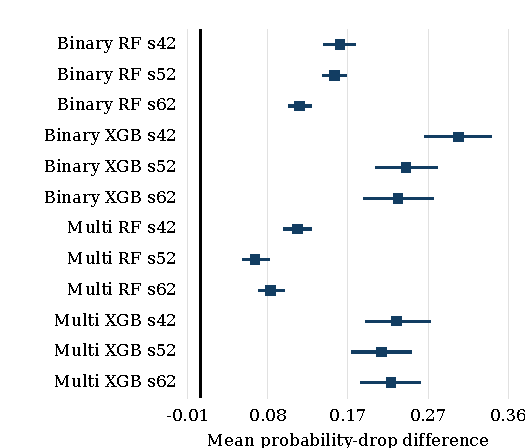
\includegraphics[width=\columnwidth]{figures/paired-1.pdf}
\caption{GeNIS paired connection-group mean differences with 95\% bootstrap intervals. Blue denotes Holm-adjusted directional p \ensuremath{<} 0.05; gray denotes non-significance. Each row is one model seed on the frozen split.}
\label{fig:1}
\end{figure}
\begin{figure}[!t]\centering
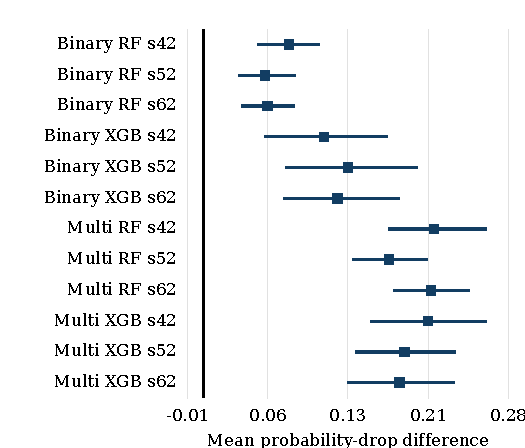
\includegraphics[width=\columnwidth]{figures/paired-2.pdf}
\caption{Gotham paired connection-group mean differences with 95\% bootstrap intervals. Blue denotes Holm-adjusted directional p \ensuremath{<} 0.05; gray denotes non-significance. Each row is one model seed on the frozen split.}
\label{fig:2}
\end{figure}
\begin{table}[!t]\centering
\caption{Paired differences across three model seeds}
\label{tab:5}
\footnotesize\setlength{\tabcolsep}{2pt}\renewcommand{\arraystretch}{1.10}
\begin{tabular}{>{\centering\arraybackslash}p{\dimexpr 0.17000\columnwidth-2\tabcolsep\relax}>{\centering\arraybackslash}p{\dimexpr 0.22000\columnwidth-2\tabcolsep\relax}>{\centering\arraybackslash}p{\dimexpr 0.18000\columnwidth-2\tabcolsep\relax}>{\centering\arraybackslash}p{\dimexpr 0.29000\columnwidth-2\tabcolsep\relax}>{\centering\arraybackslash}p{\dimexpr 0.14000\columnwidth-2\tabcolsep\relax}}\toprule
\textbf{Dataset} & \textbf{Task / model} & \textbf{Groups range} & \textbf{Mean delta range} & \textbf{Sig. / 3} \\\midrule
GeNIS & Binary RF & 93-93 & 0.117 to 0.165 & 3 / 3 \\
GeNIS & Binary XGB & 93-94 & 0.234 to 0.306 & 3 / 3 \\
GeNIS & Multi RF & 95-95 & 0.065 to 0.115 & 3 / 3 \\
GeNIS & Multi XGB & 95-95 & 0.215 to 0.232 & 3 / 3 \\
Gotham & Binary RF & 57-57 & 0.057 to 0.079 & 3 / 3 \\
Gotham & Binary XGB & 57-57 & 0.111 to 0.134 & 3 / 3 \\
Gotham & Multi RF & 63-63 & 0.172 to 0.213 & 3 / 3 \\
Gotham & Multi XGB & 63-63 & 0.182 to 0.208 & 3 / 3 \\
\bottomrule\end{tabular}\end{table}
\begin{table}[!t]\centering
\caption{Top-ranked masking relative to random control}
\label{tab:6}
\footnotesize\setlength{\tabcolsep}{2pt}\renewcommand{\arraystretch}{1.10}
\begin{tabular}{>{\centering\arraybackslash}p{\dimexpr 0.18000\columnwidth-2\tabcolsep\relax}>{\centering\arraybackslash}p{\dimexpr 0.21000\columnwidth-2\tabcolsep\relax}>{\centering\arraybackslash}p{\dimexpr 0.18000\columnwidth-2\tabcolsep\relax}>{\centering\arraybackslash}p{\dimexpr 0.18000\columnwidth-2\tabcolsep\relax}>{\centering\arraybackslash}p{\dimexpr 0.25000\columnwidth-2\tabcolsep\relax}}\toprule
\textbf{Dataset} & \textbf{Explainer} & \textbf{Positive lift / n} & \textbf{CI + Holm / n} & \textbf{Lift range} \\\midrule
GeNIS & LIME & 12/12 & 12/12 & 0.033 to 0.231 \\
GeNIS & TreeSHAP & 12/12 & 12/12 & 0.156 to 0.393 \\
Gotham & LIME & 12/12 & 8/12 & 0.015 to 0.307 \\
Gotham & TreeSHAP & 12/12 & 12/12 & 0.104 to 0.494 \\
\bottomrule\end{tabular}\end{table}
Table VI asks whether the ranking is informative under the same synthetic intervention. CI + Holm requires a positive lower 95\% group-bootstrap bound together with Holm-adjusted directional p \ensuremath{<} 0.05. Every top-minus-random hypothesis is adjusted in the 48-test family. 4 contexts (Gotham binary LIME) have positive mean lift and significant directional tests but intervals that cross zero, so they fail the combined criterion. Bottom-ranked scores remain in the artifacts as a descriptive check. An explainer comparison alone cannot show that either ranking improves over a random ranking.

\subsection{Latency, neighborhood similarity, and feature reduction}
\begin{table}[!t]\centering
\caption{Mean of three context medians and cosine means}
\label{tab:7}
\footnotesize\setlength{\tabcolsep}{2pt}\renewcommand{\arraystretch}{1.10}
\begin{tabular}{>{\centering\arraybackslash}p{\dimexpr 0.18000\columnwidth-2\tabcolsep\relax}>{\centering\arraybackslash}p{\dimexpr 0.23000\columnwidth-2\tabcolsep\relax}>{\centering\arraybackslash}p{\dimexpr 0.30000\columnwidth-2\tabcolsep\relax}>{\centering\arraybackslash}p{\dimexpr 0.29000\columnwidth-2\tabcolsep\relax}}\toprule
\textbf{Dataset} & \textbf{Task / model} & \textbf{SHAP / LIME ms} & \textbf{SHAP / LIME cosine} \\\midrule
GeNIS & Binary RF & 1.62 / 50.49 & 0.953 / 0.809 \\
GeNIS & Binary XGB & 0.99 / 26.16 & 0.956 / 0.870 \\
GeNIS & Multi RF & 2.59 / 66.68 & 0.970 / 0.683 \\
GeNIS & Multi XGB & 2.07 / 35.56 & 0.954 / 0.566 \\
Gotham & Binary RF & 2.93 / 42.04 & 0.992 / 0.922 \\
Gotham & Binary XGB & 1.15 / 8.80 & 0.981 / 0.860 \\
Gotham & Multi RF & 13.47 / 33.03 & 0.987 / 0.924 \\
Gotham & Multi XGB & 5.75 / 10.05 & 0.982 / 0.871 \\
\bottomrule\end{tabular}\end{table}
Table VII keeps each dataset/task/model context visible rather than combining correlated rows into one inferential claim. Timing excludes explainer construction and the complete IDS path, and background project-job contention was not controlled; the artifact additionally saves p90, p95, p99, throughput, top-5 overlap, and LIME repeatability. The reciprocal call-time throughput is not production IDS throughput. Neighborhood similarity depends on the chosen comparison set and representation, so it should not be called adversarial robustness.

\begin{table}[!t]\centering
\caption{Feature ablation; legacy label-union macro-f1}
\label{tab:8}
\footnotesize\setlength{\tabcolsep}{2pt}\renewcommand{\arraystretch}{1.10}
\begin{tabular}{>{\centering\arraybackslash}p{\dimexpr 0.16000\columnwidth-2\tabcolsep\relax}>{\centering\arraybackslash}p{\dimexpr 0.24000\columnwidth-2\tabcolsep\relax}>{\centering\arraybackslash}p{\dimexpr 0.15000\columnwidth-2\tabcolsep\relax}>{\centering\arraybackslash}p{\dimexpr 0.15000\columnwidth-2\tabcolsep\relax}>{\centering\arraybackslash}p{\dimexpr 0.15000\columnwidth-2\tabcolsep\relax}>{\centering\arraybackslash}p{\dimexpr 0.15000\columnwidth-2\tabcolsep\relax}}\toprule
\textbf{Dataset} & \textbf{Task / model} & \textbf{5 features} & \textbf{10 features} & \textbf{20 features} & \textbf{All} \\\midrule
GeNIS & Binary RF & 0.9998 & 0.9998 & 0.9998 & 0.9998 \\
GeNIS & Binary XGB & 0.9987 & 0.9998 & 0.9998 & 1.0000 \\
GeNIS & Multi RF & 0.9996 & 0.9996 & 0.9996 & 0.9997 \\
GeNIS & Multi XGB & 0.9888 & 0.9999 & 0.9999 & 1.0000 \\
Gotham & Binary RF & 0.9934 & 1.0000 & N/A & 1.0000 \\
Gotham & Binary XGB & 0.9946 & 0.9994 & N/A & 0.9999 \\
Gotham & Multi RF & 0.7630 & 0.8242 & N/A & 0.8238 \\
Gotham & Multi XGB & 0.4809 & 0.7661 & N/A & 0.8674 \\
\bottomrule\end{tabular}\end{table}
Feature reduction results are exploratory seed-42 refits and use the default true/predicted-label union macro-F1, which can include a predicted training-only class. They therefore use a different label averaging definition from Table II. N/A means the nominal subset exceeds the available predictor count. Requested counts are capped in the raw experiment, so repeated full-count rows are displayed once under All. The ranking is fitted on training data, but comparing multiple subsets on the held-out test set does not constitute independently validated feature selection. Any final subset should be fixed and confirmed on a new holdout. SHAP latency measured in this ablation is a small batched probe and is not directly interchangeable with Table VII's warmed single-record timings.

\subsection{Sensitivity and calibration audits}
Additional seed-42 audits evaluate binary calibration on the test cohort (Table IX), weighted versus unweighted fitting, TreeSHAP masking under five baselines on 12 diagnostic records, and LIME perturbation budgets 100, 350, and 700 on six records with five repeats (Table X). These small sensitivity cohorts provide descriptive checks; they are not independent confirmatory studies or a replacement for the paired group-level primary endpoint.

\begin{table}[!t]\centering
\caption{Binary seed-42 calibration on the capped cohort}
\label{tab:9}
\footnotesize\setlength{\tabcolsep}{2pt}\renewcommand{\arraystretch}{1.10}
\begin{tabular}{>{\centering\arraybackslash}p{\dimexpr 0.48000\columnwidth-2\tabcolsep\relax}>{\centering\arraybackslash}p{\dimexpr 0.26000\columnwidth-2\tabcolsep\relax}>{\centering\arraybackslash}p{\dimexpr 0.26000\columnwidth-2\tabcolsep\relax}}\toprule
\textbf{Dataset / model} & \textbf{Brier} & \textbf{10-bin ECE} \\\midrule
GeNIS RF & 0.0001 & 0.0010 \\
GeNIS XGB & 0.0002 & 0.0002 \\
Gotham RF & 0.0001 & 0.0026 \\
Gotham XGB & 0.0000 & 0.0002 \\
\bottomrule\end{tabular}\end{table}
Across the eight contexts, descriptive TreeSHAP mean deletion scores under the masking alternatives are marginal training row: 0.360; nearest opposite prediction: 0.539; nearest same prediction: -0.005; training median mode: 0.423; zero: 0.290. This pooling is a sensitivity summary only. Baseline-dependent scores reinforce that the masking intervention is part of the measured construct.

\begin{table}[!t]\centering
\caption{Descriptive lime budget audit, contexts pooled}
\label{tab:10}
\footnotesize\setlength{\tabcolsep}{2pt}\renewcommand{\arraystretch}{1.10}
\begin{tabular}{>{\centering\arraybackslash}p{\dimexpr 0.24000\columnwidth-2\tabcolsep\relax}>{\centering\arraybackslash}p{\dimexpr 0.25000\columnwidth-2\tabcolsep\relax}>{\centering\arraybackslash}p{\dimexpr 0.25000\columnwidth-2\tabcolsep\relax}>{\centering\arraybackslash}p{\dimexpr 0.26000\columnwidth-2\tabcolsep\relax}}\toprule
\textbf{LIME samples} & \textbf{Deletion} & \textbf{Repeat cosine} & \textbf{Median ms} \\\midrule
100 & 0.222 & 0.702 & 26.70 \\
350 & 0.232 & 0.834 & 29.84 \\
700 & 0.252 & 0.872 & 33.56 \\
\bottomrule\end{tabular}\end{table}
Class-weighted minus unweighted test-supported-label macro-F1 varies from -0.0043 to 0.0000 across seed-42 contexts. Calibration values apply to the known-label capped test cohort; they do not estimate calibration at natural deployment prevalence. The LIME budget audit reuses seeds and records and is presented without a pooled significance claim.

\subsection{Post-hoc sign, influence and pattern-exclusion checks}
A separately labelled post-hoc sensitivity analysis reproduces all 24 original paired means and group counts. Exact two-sided sign tests on connection-level differences, excluding absolute differences at most 1e-12, favor TreeSHAP in 24/24 contexts after Holm correction within this separate family. Removing any one explained connection reverses the mean sign in 0/24 contexts. The sign test targets direction frequency, not the mean endpoint, and still requires sufficiently independent connection signs. Leave-one-out extrema are influence diagnostics, not confidence intervals.

\begin{table}[!t]\centering
\caption{Post-hoc seed-42 multiclass pattern sensitivity}
\label{tab:11}
\footnotesize\setlength{\tabcolsep}{2pt}\renewcommand{\arraystretch}{1.10}
\begin{tabular}{>{\centering\arraybackslash}p{\dimexpr 0.48000\columnwidth-2\tabcolsep\relax}>{\centering\arraybackslash}p{\dimexpr 0.26000\columnwidth-2\tabcolsep\relax}>{\centering\arraybackslash}p{\dimexpr 0.26000\columnwidth-2\tabcolsep\relax}}\toprule
\textbf{Dataset / model} & \textbf{Original F1} & \textbf{Pattern-excluded F1} \\\midrule
GeNIS RF & 0.9997 & 0.9997 \\
GeNIS XGB & 1.0000 & 1.0000 \\
Gotham RF & 0.8748 & 0.8639 \\
Gotham XGB & 0.8659 & 0.8562 \\
\bottomrule\end{tabular}\end{table}
A second post-hoc diagnostic excludes test records with exactly matching raw predictor vectors in training, without using labels in the matching key (GeNIS: 379 excluded and 7,275 retained; Gotham: 1,914 excluded and 24,456 retained). No model is refitted or selected. Macro-F1 keeps the original supported-test-label denominator; no supported label is lost. Table XI exposes the Gotham multiclass reduction. Reusing the saved explanation records after this exclusion retains 53-95 explained groups per context; 24/24 mean differences remain positive and 24/24 two-sided sign tests favor TreeSHAP after a separate Holm adjustment. This is a conditional selection diagnostic, not a new disjoint split or external validation; it cannot remove shared campaign or testbed mechanisms.

\subsection{Paired sensitivity to the replacement distribution}
The earlier five-reference audit evaluated only TreeSHAP on twelve records per context. To test the comparison itself, a new exploratory protocol reuses all 100 saved matched records, both saved rankings and the eight seed-42 models. It compares the original median/mode reference with two training-donor schemes. A fixed pool samples 5,000 training rows uniformly. Empirical replacement copies removed features jointly from 32 donors, using the same draws for both explainers and all budgets of a record. Nearest-donor replacement chooses 32 pool rows using retained predictors only: numeric distances use training IQR (standard deviation, then one, as fallbacks), are capped at one, and categorical predictors contribute mismatch indicators. Distances average retained predictors; labels and model outputs never select donors. Removed values are copied jointly and the 32 target probabilities averaged. This approximate conditioning sensitivity does not guarantee physically valid network traffic.

\begin{table}[!t]\centering
\caption{Replacement-specific mean treeshap-minus-lime deletion, seed 42}
\label{tab:12}
\footnotesize\setlength{\tabcolsep}{2pt}\renewcommand{\arraystretch}{1.10}
\begin{tabular}{>{\centering\arraybackslash}p{\dimexpr 0.29000\columnwidth-2\tabcolsep\relax}>{\centering\arraybackslash}p{\dimexpr 0.13000\columnwidth-2\tabcolsep\relax}>{\centering\arraybackslash}p{\dimexpr 0.13000\columnwidth-2\tabcolsep\relax}>{\centering\arraybackslash}p{\dimexpr 0.13000\columnwidth-2\tabcolsep\relax}>{\centering\arraybackslash}p{\dimexpr 0.32000\columnwidth-2\tabcolsep\relax}}\toprule
\textbf{Dataset / task / model} & \textbf{Median} & \textbf{Joint} & \textbf{Nearest} & \textbf{Nearest 95\% CI} \\\midrule
GeNIS Binary RF & 0.1653 & 0.0730 & 0.0023 & [-0.0018, 0.0079] \\
GeNIS Binary XGB & 0.3058 & 0.0696 & 0.0049 & [-0.0008, 0.0117] \\
GeNIS Multi RF & 0.1153 & 0.0983 & 0.0034 & [-0.0044, 0.0116] \\
GeNIS Multi XGB & 0.2321 & 0.2030 & 0.0109 & [0.0022, 0.0227] \\
Gotham Binary RF & 0.0791 & 0.0995 & 0.0327 & [0.0173, 0.0503] \\
Gotham Binary XGB & 0.1114 & 0.1211 & 0.0113 & [0.0013, 0.0232] \\
Gotham Multi RF & 0.2135 & 0.1471 & 0.1961 & [0.1608, 0.2355] \\
Gotham Multi XGB & 0.2079 & 0.1385 & 0.2013 & [0.1593, 0.2415] \\
\bottomrule\end{tabular}\end{table}
Original median/mode drops reproduce to a maximum absolute error of 3.33e-16. Table XII shows that the measured advantage depends strongly on replacement. GeNIS nearest-donor mean gaps are only 0.0023-0.0109, and 3/4 corresponding pointwise mean intervals cross zero. Across both datasets, nearest donors retain 8/8 positive means and 5/8 positive lower interval bounds. Exact two-sided sign tests favor TreeSHAP in 4/8 nearest contexts after Holm adjustment across the separate 24-context/scheme family; median/mode and empirical donors each have 8/8. The tests target non-tied direction frequency rather than the mean: GeNIS binary RF has 69 ties among 93 groups, while multiclass RF has 56 among 95. A positive mean, a positive interval and a significant sign test are not interchangeable findings. All schemes, including weak effects, are retained.

\subsection{Controlled LIME budget and local fit}
A second exploratory extension refits LIME explanations, not detectors. On the same 100 records in each seed-42 context, it fits a fresh default-neighborhood surrogate at 350 and 3,500 perturbations using a common per-record seed and training background. Common seeds do not guarantee nested random samples. This fresh schedule differs from the original sequential warm-up and is not a reproduction of the primary 350-draw ranking. Saved TreeSHAP and both fresh LIME rankings are evaluated with the original median/mode mask. Group bootstrap intervals and exact two-sided sign tests follow the other exploratory analyses, with Holm adjustment over eight TreeSHAP-minus-LIME-3500 and eight LIME-3500-minus-LIME-350 contrasts as one separate family.

\begin{table}[!t]\centering
\caption{Controlled lime budget: query fit and group deletion}
\label{tab:13}
\footnotesize\setlength{\tabcolsep}{2pt}\renewcommand{\arraystretch}{1.10}
\begin{tabular}{>{\centering\arraybackslash}p{\dimexpr 0.34000\columnwidth-2\tabcolsep\relax}>{\centering\arraybackslash}p{\dimexpr 0.25000\columnwidth-2\tabcolsep\relax}>{\centering\arraybackslash}p{\dimexpr 0.19000\columnwidth-2\tabcolsep\relax}>{\centering\arraybackslash}p{\dimexpr 0.22000\columnwidth-2\tabcolsep\relax}}\toprule
\textbf{Dataset / task / model} & \textbf{Fit error 350 / 3500} & \textbf{LIME budget delta} & \textbf{SHAP - LIME 3500} \\\midrule
GeNIS Binary RF & 0.165 / 0.266 & 0.007 & 0.164 \\
GeNIS Binary XGB & 0.105 / 0.173 & 0.030 & 0.281 \\
GeNIS Multi RF & 0.281 / 0.459 & 0.057 & 0.071 \\
GeNIS Multi XGB & 0.261 / 0.448 & 0.093 & 0.164 \\
Gotham Binary RF & 0.333 / 0.363 & -0.009 & 0.087 \\
Gotham Binary XGB & 0.414 / 0.432 & 0.001 & 0.109 \\
Gotham Multi RF & 0.653 / 0.694 & -0.000 & 0.205 \\
Gotham Multi XGB & 0.734 / 0.779 & 0.029 & 0.165 \\
\bottomrule\end{tabular}\end{table}
LIME-3500 mean deletion improves over LIME-350 in 6/8 contexts, with 2/8 corrected sign tests in that direction. TreeSHAP still has larger mean deletion in 8/8 contexts and positive corrected sign tests in 8/8. Yet mean absolute error at the explained input increases in 8/8 contexts; at 3,500 samples its context means range from 0.173 to 0.779 on the probability scale. Mean in-neighborhood weighted R-squared falls in 7/8. These descriptive fit scores are distinct from deletion fidelity. More draws do not guarantee an adequate surrogate or establish convergence; the observed comparison remains conditional on the chosen LIME neighborhood.

At 3,500 draws, a width grid (0.15, 0.35, 0.75 times the square root of the feature count) reuses identical sampled neighborhoods and model outputs, and reproduces the saved 0.75 fits. The narrowest width lowers mean query error in 8/8 contexts but does not eliminate large errors in Gotham multiclass. Under median/mode deletion, TreeSHAP mean gaps remain positive in 16/16 new contrasts, with 13/16 positive signs after separate Holm correction. No width is selected on test performance. Weighted fit scores use different kernel weights and are not a common test distribution.

\subsection{Source-file transfer with shared groups purged}
A separate stress test partitions the union of the original prepared rows by source instead of by connection alone. It holds out each of eight GeNIS scenario CSVs. For Gotham, each of eight bundles holds out one attack-bearing source and an assigned subset of the 57 benign-only sources. Stable SHA-256 filename order fixes the attack-source order and round-robin benign assignments before fitting. All 65 represented Gotham CSVs are held out once; thirteen acquired files have no rows in the capped cohort. All remaining training rows whose global connection keys occur anywhere in the held-out sources are purged. No source or group overlaps within a fold. Raw member hashes and row identities are verified while restoring the fifteen GeNIS and one Gotham candidate predictors removed as constants in the original split. Constant filtering, imputation and category encoding then fit on each fold's training rows alone.

For each of sixteen folds, the same binary/multiclass RF and XGB hyperparameters and training-weight policies are refitted at seed 42, for 64 fits; majority and depth-five trees remain baselines. Every held-out class with test support contributes to macro-F1, including labels missing from the training vocabulary. A separate seen-label score restricts both test rows and averaging labels. The two explainers process 50 matched class/error diagnostic records per refit, with the original median/mode mask, random control and 350 LIME perturbations. We report mean differences descriptively: the folds share training data and can reuse connection groups across different test sources, so the 64 contexts are not pooled for significance inference.

\begin{table}[!t]\centering
\caption{Source holdout: all-test-label macro-f1 and paired deletion}
\label{tab:14}
\footnotesize\setlength{\tabcolsep}{2pt}\renewcommand{\arraystretch}{1.10}
\begin{tabular}{>{\centering\arraybackslash}p{\dimexpr 0.30000\columnwidth-2\tabcolsep\relax}>{\centering\arraybackslash}p{\dimexpr 0.32000\columnwidth-2\tabcolsep\relax}>{\centering\arraybackslash}p{\dimexpr 0.25000\columnwidth-2\tabcolsep\relax}>{\centering\arraybackslash}p{\dimexpr 0.13000\columnwidth-2\tabcolsep\relax}}\toprule
\textbf{Dataset / task / model} & \textbf{F1 mean [range]} & \textbf{SHAP - LIME range} & \textbf{Positive / 8} \\\midrule
GeNIS Binary RF & 0.916 [0.373, 1.000] & -0.017 to 0.068 & 7 \\
GeNIS Binary XGB & 0.702 [0.333, 0.991] & 0.057 to 0.196 & 8 \\
GeNIS Multi RF & 0.831 [0.471, 0.999] & -0.005 to 0.156 & 7 \\
GeNIS Multi XGB & 0.735 [0.465, 0.998] & 0.196 to 0.415 & 8 \\
Gotham Binary RF & 0.949 [0.593, 1.000] & 0.015 to 0.134 & 8 \\
Gotham Binary XGB & 0.916 [0.591, 1.000] & 0.055 to 0.274 & 8 \\
Gotham Multi RF & 0.872 [0.666, 0.942] & 0.138 to 0.239 & 8 \\
Gotham Multi XGB & 0.880 [0.654, 0.964] & 0.120 to 0.275 & 8 \\
\bottomrule\end{tabular}\end{table}
The source-held-out scores in Table XIV vary substantially even when all test labels appear in training. In GeNIS scenario 6, binary XGB macro-F1 is 0.3327 and the attack false-negative rate is 84.46\%. Its multiclass model has recall 0.000 on 3,853 brute-force records despite 6,147 same-label training records. Gotham's combined-cycle-1 fold additionally contains 14,242 records from labels absent in training (CoAP Amplification and UDP Scan), which contribute zero recall. TreeSHAP-minus-LIME mean deletion is positive in 62/64 contexts and negative in 2/64 under this mask. This alternative split changes source membership, group purging, train size and test class mix jointly; their individual effects are not identified. The experiment is within the original two testbeds, not an external capture validation.

\subsection{Uncapped source files and independent capture}
Without refitting, we score the same 64 source-holdout detectors on the complete assigned files: eight GeNIS scenarios and 65 Gotham sources. Gotham files absent from the capped assignment are outside this comparison. We exclude Unknown and any additional raw test rows whose connection keys match capped training, then replay full confusion matrices. The original sampled training sets remain fixed. This tests a change in test coverage and recorded prevalence together, not the effect of increasing training size.

Uncapped scoring retains 3,012,335 GeNIS and 34,929,055 Gotham records after label and connection exclusions. Binary macro-F1 spans 0.042-1.000 across GeNIS fold-model contexts and 0.764-1.000 across Gotham contexts.

On the expanded GeNIS scenario 6 test, binary XGBoost misses 10,003 of 11,995 attack records and flags 15 of 33,670 benign records. Capped and uncapped results use different test compositions and should not be interpreted as a causal sample-size effect.

For independent capture transfer, fresh binary RF and XGB models fit only the original GeNIS training partition. The official OCPP 1.6 charging-network dataset \cite{ref37} supplies 4,415 externally captured flows from both provider Combined partitions, kept entirely out of fitting and threshold selection. One fixed feature set uses protocol and unordered TCP/UDP ports; the other adds duration in seconds and total packets. Units and directions are harmonized, but Argus and CICFlowMeter may segment traffic differently. The external release is provider-balanced by category (883 benign and 3,532 attack-labeled flows); it cannot estimate operational prevalence or alert volume.

\begin{table}[!t]\centering
\caption{Independent ocpp transfer; misses of 3,532, false alarms of 883}
\label{tab:15}
\footnotesize\setlength{\tabcolsep}{2pt}\renewcommand{\arraystretch}{1.10}
\begin{tabular}{>{\centering\arraybackslash}p{\dimexpr 0.32000\columnwidth-2\tabcolsep\relax}>{\centering\arraybackslash}p{\dimexpr 0.16000\columnwidth-2\tabcolsep\relax}>{\centering\arraybackslash}p{\dimexpr 0.16000\columnwidth-2\tabcolsep\relax}>{\centering\arraybackslash}p{\dimexpr 0.16000\columnwidth-2\tabcolsep\relax}>{\centering\arraybackslash}p{\dimexpr 0.20000\columnwidth-2\tabcolsep\relax}}\toprule
\textbf{Set / model} & \textbf{GeNIS F1} & \textbf{OCPP F1} & \textbf{Missed} & \textbf{False alarms} \\\midrule
Transport RF & 0.995 & 0.874 & 5 & 303 \\
Transport XGB & 0.995 & 0.865 & 2 & 325 \\
Plus volume RF & 0.999 & 0.637 & 821 & 381 \\
Plus volume XGB & 0.999 & 0.657 & 807 & 338 \\
\bottomrule\end{tabular}\end{table}
Protocol/port models miss only two to five attack-labeled flows but flag 303-325 benign flows. Adding duration and packet count raises source-test macro-F1 yet lowers external macro-F1 for both models; it misses 807-821 attack-labeled flows, mainly unauthorized-access examples. This is transfer of reduced-feature binary classifiers to one independent testbed, not validation of the original full-feature models, multiclass taxonomies, or explanation fidelity.

\subsection{Training-size sensitivity on unseen GeNIS scenarios}
We tested binary detector sensitivity to training size in the eight GeNIS source holdouts. Uniform nested training samples of 10,000, 40,000, and 160,000 rows per fold come from the other seven files after excluding every row whose FlowID appears anywhere in the held-out file. Raw class mix is preserved in expectation, and the original model weighting, settings, and seed 42 are fixed. Preprocessing is fitted separately on each training prefix. Within each fold, all sizes score exactly the same complete source file. Together these files contain 3,087,981 test rows.
Random Forest equal-scenario mean macro-F1 is 0.454, 0.542, 0.531 at 10,000, 40,000, and 160,000 rows. The largest cohort improves over the smallest in 6/8 scenarios and declines in 1/8 (paired change -0.036 to +0.312). XGBoost equal-scenario mean macro-F1 is 0.597, 0.528, 0.543 at 10,000, 40,000, and 160,000 rows. The largest cohort improves over the smallest in 5/8 scenarios and declines in 3/8 (paired change -0.807 to +0.155).
In GeNIS scenario 4, XGBoost misses 4, 771,164, and 785,849 of 788,426 attacks as training size increases. The corresponding training cohorts contain only 12, 45, and 155 benign rows. This is a post-hoc, descriptive GeNIS analysis with overlapping training pools and one nested draw per scenario. Larger samples can add coverage of different connections and attack categories. This experiment addresses binary detection under scenario separation within one testbed.
\subsection{Protocol shortcut controls and base-rate sensitivity}
To test whether the reduced-feature transfer result required a tree ensemble, we ran two exploratory controls on the same source and external cohorts. A lookup assigns the training-majority binary label for the observed protocol or exact protocol and unordered port pair. Unseen pairs back off to protocol. Ties and unseen protocols predict benign. The rules use unweighted GeNIS training counts. The external capture was already inspected in the earlier study, so the comparison is retrospective.
On OCPP, the protocol-only and pair rules reach macro-F1 of 0.920 and 0.918, versus 0.865 to 0.874 for the three-field trees. The protocol rule misses 0 of 3,532 attacks and flags 206 of 883 benign flows. All 3,532 labeled OCPP attacks use TCP. Exact pairs seen in GeNIS training cover only 527 of 4,415 OCPP flows. This capture rewards protocol-label association and offers limited evidence that the trees transfer attack behavior. The control does not identify which features drive the original full models.
Restricting OCPP to TCP retains all 3,532 attacks and 162 benign flows. The protocol rule now flags all benign flows, and both three-field trees flag 161 of 162. Their TCP-only macro-F1 is 0.494 to 0.495. For this post-hoc diagnostic, the original source-only tree fits were rebuilt and required to match the saved full-capture error counts before their TCP-only results were reported.
Under a hypothetical 1 percent attack prevalence and fixed observed class-conditional rates, positive predictive value is 4.2\% for the protocol rule and 2.7\% to 2.9\% for the three-field trees. The corresponding expected false-alert counts per 10,000 records are 2,310 and 3,397 to 3,644. These are base-rate sensitivity calculations \cite{ref38}. They assume stable conditional rates and count record alerts, so they do not estimate production analyst workload.
\subsection{Independent protocol-matched TCP transfer}
We added an independent protocol-matched evaluation using the provider's PDMFC v1 capture \cite{ref39}, exported from pfSense traffic with CICFlowMeter. We verify the complete CSV against the publisher checksum and use its populated lowercase annotation field. Models, weighting, preprocessing and decisions are carried over from the GeNIS-only transfer configuration. The rebuilt fits reproduce the saved OCPP full-capture and TCP confusion counts before PDMFC scoring. The primary diagnostic includes all TCP flows in the release.

The TCP cohort contains 37,226 attack and 12,006 benign flows. Random Forest and XGBoost with protocol and ports raise 11,882 and 11,834 false alarms (99.0\% and 98.6\%) and miss 182 and 123 attacks, respectively. The protocol-only control flags 12,006 benign flows and misses 0 attacks. Exact unordered TCP port pairs carrying both labels cover 161 flows (109 attack and 52 benign). The transport trees flag 52 of those benign flows.

PDMFC contributes one separately collected file with 49,515 flows. The provider labels 35,888 of its TCP attacks as Web Attack. The provider labels and error rates are descriptive of this release. Protocol matching does not control endpoints, traffic mix or capture conditions, and repeated flows within the capture are not independent replications.

\section{Discussion and threats to validity}
The refreshed evidence addresses the missing local conversion history by making the source-to-cohort transformation inspectable and rerunnable. It does not retrospectively recover the legacy parquet provenance. Source snapshots and hashes fix the consumed author files and executed transformations, while the narrower Gotham member-verification scope remains a declared limitation. CRC32 detects transfer or extraction inconsistency; it is not a publisher-signed cryptographic authenticity proof.

The primary group split prevents the chosen connection keys from crossing partitions but does not separate source files. The secondary holdout adds that separation and purges shared connection keys, while GeNIS scenarios can still share generation mechanisms and Gotham source files can share a virtual testbed or campaign. Neither original within-testbed design is forward-in-time or cross-network; the separate OCPP and PDMFC captures test reduced-feature binary transfer. The source analysis exposes weak transfer within the observed cohorts; it does not estimate an external site's error rates. Equal feature patterns can still occur in different groups and sources.

The class cap changes prevalence and can underrepresent rare attack diversity. Unknown-labelled packets are outside both supervised tasks. A label confined to one group cannot support an independent test claim; the supported-class macro-F1 is restricted to labels present in test. Five predictive seeds share one preparation seed and one split; they do not explore split uncertainty. Explanation sampling prioritizes error types, and the inferential population is the explained groups represented by this selection rather than every packet in the full dataset. Group means reduce within-key dependence but do not remove all dependence across groups or model seeds.

The directional TreeSHAP-greater test permits checking that specific hypothesis; a reverse claim requires a separately specified analysis. Bootstrap intervals are per context and are not simultaneous confidence intervals, whereas Holm controls the reported hypothesis families. The default TreeSHAP value function and LIME's discretized local surrogate can respond differently to correlated and categorical predictors. Masking by a mixed median/mode vector can create off-manifold combinations, so a larger deletion drop is a protocol-specific ranking result.

This work has no participant study, production monitoring, packet-capture throughput benchmark, drift test, or attack intervention study. Gaspar \emph{et al.} \cite{ref14} include a perceived-interpretability survey; our work has no corresponding human evidence. Neither our deletion results nor that survey establish operational alert cost, current attack coverage, or adversarial safety. A stronger next evaluation would freeze the chosen configuration, use a separately captured device/scenario/time holdout, retain natural prevalence for operational calibration, and measure analyst decisions with a pre-specified human study.

\textbf{Implications for detector review:} In GeNIS scenario 6, the two ensembles and the depth-five tree each raise zero false alarms over 1,266 benign records, yet miss 3,643, 3,854 and 3,859 of 4,563 attack records, respectively. The failure is shared across model families. Report missed attacks and false alarms with denominators on held-out sources before judging detector coverage. For explanations, report original-query surrogate error separately from deletion and show sensitivity to alternative replacements. These checks inform review priorities; they have not been validated as an analyst workflow.

\section{Reproducibility and reporting status}
The executed environment uses Python 3.12.14, scikit-learn 1.6.1, XGBoost 3.0.2, SHAP 0.47.2, and LIME 0.2.0.1. The project saves author-record metadata, acquisition and per-member hashes, exclusions, source row counts, class counts, split and overlap audits, prepared parquet hashes, source snapshots, fitted seed-42 models, and per-context checkpoints. The configuration and source hashes in run\_manifest.json define this run. Artifact verification checks coverage and internal consistency; it is not independent external replication.

A clean rerun begins with the official acquisition scripts, then deterministic preparation, the recent-data benchmark, and artifact verification. It requires the author data downloads and the pinned requirements. The benchmark caps are part of the experiment and should not be silently replaced with full-data or per-file caps. No repository release, archival DOI, or externally executed replication is claimed in this draft.

\textbf{AI assistance disclosure:} OpenAI Codex assisted with source acquisition tooling, data auditing, experiment orchestration, and manuscript drafting.

\section{Conclusion}
Source holdouts expose missed attacks that aggregate scores can hide. Increasing the GeNIS training cohort from 10,000 to 160,000 rows improves some scenarios but does not consistently improve binary detection. The reduced-feature detectors also flag nearly all benign TCP flows in two independent captures. Separately, TreeSHAP leads LIME under median/mode deletion in all 24 primary contexts, but retained-feature donor replacement weakens the GeNIS gaps. These findings concern the evaluated detectors, captures and replacement rules. External explanation fidelity and analyst decisions remain untested.

\begin{thebibliography}{39}
\bibitem{ref1} M. Silva, D. Pinto, J. Vitorino, J. Gonçalves, E. Maia, and I. Praça, "GeNIS: GECAD Network Intrusion Scenarios," Zenodo, ver. 1.0.0, Feb. 24, 2025, doi: \href{https://doi.org/10.5281/zenodo.14919237}{10.5281/zenodo.14919237}.
\bibitem{ref2} M. Silva, D. Pinto, J. Vitorino, J. Gonçalves, E. Maia, and I. Praça, "GeNIS: A modular dataset for network intrusion detection and classification," \emph{Data in Brief}, vol. 60, art. no. 111487, Jun. 2025, doi: \href{https://doi.org/10.1016/j.dib.2025.111487}{10.1016/j.dib.2025.111487}.
\bibitem{ref3} O. Belarbi, T. Spyridopoulos, E. Anthi, O. Rana, P. Carnelli, and A. Khan, "A Device-Level IoT Network Traffic Dataset with Distributed Capture and Non-IID Characteristics," Zenodo, ver. v1, Feb. 5, 2025, doi: \href{https://doi.org/10.5281/zenodo.14502760}{10.5281/zenodo.14502760}.
\bibitem{ref4} O. Belarbi, T. Spyridopoulos, E. Anthi, O. Rana, P. Carnelli, and A. Khan, "Gotham Dataset 2025: A Reproducible Large-Scale IoT Network Dataset for Intrusion Detection and Security Research," arXiv:2502.03134, ver. 1, Feb. 5, 2025, doi: \href{https://doi.org/10.48550/arXiv.2502.03134}{10.48550/arXiv.2502.03134}.
\bibitem{ref5} L. Breiman, "Random forests," \emph{Machine Learning}, vol. 45, no. 1, pp. 5-32, 2001, doi: \href{https://doi.org/10.1023/A:1010933404324}{10.1023/A:1010933404324}.
\bibitem{ref6} T. Chen and C. Guestrin, "XGBoost: A scalable tree boosting system," in \emph{Proc. ACM SIGKDD}, 2016, pp. 785-794, doi: \href{https://doi.org/10.1145/2939672.2939785}{10.1145/2939672.2939785}.
\bibitem{ref7} S. M. Lundberg and S.-I. Lee, "A unified approach to interpreting model predictions," in \emph{Advances in Neural Information Processing Systems}, vol. 30, 2017. [Online]. Available: \href{https://proceedings.neurips.cc/paper/2017/hash/8a20a8621978632d76c43dfd28b67767-Abstract.html}{NeurIPS proceedings}.
\bibitem{ref8} S. M. Lundberg \emph{et al.}, "From local explanations to global understanding with explainable AI for trees," \emph{Nature Machine Intelligence}, vol. 2, pp. 56-67, 2020, doi: \href{https://doi.org/10.1038/s42256-019-0138-9}{10.1038/s42256-019-0138-9}.
\bibitem{ref9} M. T. Ribeiro, S. Singh, and C. Guestrin, "Why should I trust you?": Explaining the predictions of any classifier, in \emph{Proc. ACM SIGKDD}, 2016, pp. 1135-1144, doi: \href{https://doi.org/10.1145/2939672.2939778}{10.1145/2939672.2939778}.
\bibitem{ref10} C.-K. Yeh, C.-Y. Hsieh, A. S. Suggala, D. I. Inouye, and P. Ravikumar, "On the (in)fidelity and sensitivity of explanations," in \emph{Advances in Neural Information Processing Systems}, vol. 32, 2019. [Online]. Available: \href{https://proceedings.neurips.cc/paper/2019/hash/a7471fdc77b3435276507cc8f2dc2569-Abstract.html}{NeurIPS proceedings}.
\bibitem{ref11} J. Adebayo, J. Gilmer, M. Muelly, I. Goodfellow, M. Hardt, and B. Kim, "Sanity checks for saliency maps," in \emph{Advances in Neural Information Processing Systems}, vol. 31, 2018. [Online]. Available: \href{https://proceedings.neurips.cc/paper/2018/hash/294a8ed24b1ad22ec2e7efea049b8737-Abstract.html}{NeurIPS proceedings}.
\bibitem{ref12} S. Neupane \emph{et al.}, "Explainable intrusion detection systems (X-IDS): A survey of current methods, challenges, and opportunities," \emph{IEEE Access}, vol. 10, pp. 112392-112415, 2022, doi: \href{https://doi.org/10.1109/ACCESS.2022.3216617}{10.1109/ACCESS.2022.3216617}.
\bibitem{ref13} S. Mane and D. Rao, "Explaining network intrusion detection system using explainable AI framework," arXiv:2103.07110, ver. 1, Mar. 12, 2021, doi: \href{https://doi.org/10.48550/arXiv.2103.07110}{10.48550/arXiv.2103.07110}.
\bibitem{ref14} D. Gaspar, P. Silva, and C. Silva, "Explainable AI for intrusion detection systems: LIME and SHAP applicability on multi-layer perceptron," \emph{IEEE Access}, vol. 12, pp. 30164-30175, 2024, doi: \href{https://doi.org/10.1109/ACCESS.2024.3368377}{10.1109/ACCESS.2024.3368377}.
\bibitem{ref15} A. Warnecke, D. Arp, C. Wressnegger, and K. Rieck, "Evaluating explanation methods for deep learning in security," in \emph{Proc. IEEE Eur. Symp. Security and Privacy (EuroS\&P)}, 2020, pp. 158-174, doi: \href{https://doi.org/10.1109/EuroSP48549.2020.00018}{10.1109/EuroSP48549.2020.00018}.
\bibitem{ref16} O. Arreche, T. R. Guntur, J. W. Roberts, and M. Abdallah, "E-XAI: Evaluating black-box explainable AI frameworks for network intrusion detection," \emph{IEEE Access}, vol. 12, pp. 23954-23988, 2024, doi: \href{https://doi.org/10.1109/ACCESS.2024.3365140}{10.1109/ACCESS.2024.3365140}.
\bibitem{ref17} R. Kalakoti, R. Vaarandi, H. Bahsi, and S. Nomm, "Evaluating explainable AI for deep learning-based network intrusion detection system alert classification," arXiv:2506.07882, ver. 1, 2025. [Online]. Available: \href{https://arxiv.org/abs/2506.07882v1}{arXiv preprint}.
\bibitem{ref18} A. Kumar and V. L. L. Thing, "Evaluating the explainability of state-of-the-art machine learning-based IoT network intrusion detection systems," arXiv:2408.14040, ver. 1, 2024. [Online]. Available: \href{https://arxiv.org/abs/2408.14040v1}{arXiv preprint}.
\bibitem{ref19} P. Hermosilla, S. Berrios, and H. Allende-Cid, "Explainable AI for forensic analysis: A comparative study of SHAP and LIME in intrusion detection models," \emph{Applied Sciences}, vol. 15, no. 13, art. 7329, 2025, doi: \href{https://doi.org/10.3390/app15137329}{10.3390/app15137329}.
\bibitem{ref20} B. Nugraha, A. V. Jnanashree, and T. Bauschert, "A versatile XAI-based framework for efficient and explainable intrusion detection systems," \emph{Annals of Telecommunications}, vol. 80, pp. 1095-1120, 2025, doi: \href{https://doi.org/10.1007/s12243-025-01118-9}{10.1007/s12243-025-01118-9}.
\bibitem{ref21} D. Arp \emph{et al.}, "Dos and don'ts of machine learning in computer security," in \emph{Proc. USENIX Security}, 2022, pp. 3971-3988. [Online]. Available: \href{https://www.usenix.org/conference/usenixsecurity22/presentation/arp}{USENIX proceedings}.
\bibitem{ref22} G. Engelen, V. Rimmer, and W. Joosen, "Troubleshooting an intrusion detection dataset: The CICIDS2017 case study," in \emph{Proc. IEEE Security and Privacy Workshops}, 2021, pp. 7-12, doi: \href{https://doi.org/10.1109/SPW53761.2021.00009}{10.1109/SPW53761.2021.00009}.
\bibitem{ref23} C. Rudin, "Stop explaining black box machine learning models for high stakes decisions and use interpretable models instead," \emph{Nature Machine Intelligence}, vol. 1, pp. 206-215, 2019, doi: \href{https://doi.org/10.1038/s42256-019-0048-x}{10.1038/s42256-019-0048-x}.
\bibitem{ref24} S. Krishna, T. Han, A. Gu, J. Pombra, S. Jabbari, S. Wu, and H. Lakkaraju, "The disagreement problem in explainable machine learning: A practitioner's perspective," arXiv:2202.01602, ver. 1, 2022. [Online]. Available: \href{https://arxiv.org/abs/2202.01602v1}{arXiv preprint}.
\bibitem{ref25} D. Slack, S. Hilgard, E. Jia, S. Singh, and H. Lakkaraju, "Fooling LIME and SHAP: Adversarial attacks on post hoc explanation methods," in \emph{Proc. AAAI/ACM AIES}, 2020, pp. 180-186, doi: \href{https://doi.org/10.1145/3375627.3375830}{10.1145/3375627.3375830}.
\bibitem{ref26} P. Hase, H. Xie, and M. Bansal, "The out-of-distribution problem in explainability and search methods for feature importance explanations," in \emph{Advances in Neural Information Processing Systems}, vol. 34, 2021. [Online]. Available: \href{https://arxiv.org/abs/2106.00786}{Author preprint}.
\bibitem{ref27} K. Aas, M. Jullum, and A. Loland, "Explaining individual predictions when features are dependent: More accurate approximations to Shapley values," \emph{Artificial Intelligence}, vol. 298, art. 103502, 2021, doi: \href{https://doi.org/10.1016/j.artint.2021.103502}{10.1016/j.artint.2021.103502}.
\bibitem{ref28} M. Sundararajan and A. Najmi, "The many Shapley values for model explanation," in \emph{Proc. ICML}, PMLR, vol. 119, 2020, pp. 9269-9278. [Online]. Available: \href{https://proceedings.mlr.press/v119/sundararajan20b.html}{PMLR proceedings}.
\bibitem{ref29} C. Agarwal \emph{et al.}, "OpenXAI: Towards a transparent evaluation of post hoc model explanations," in \emph{Advances in Neural Information Processing Systems}, vol. 35, 2022. [Online]. Available: \href{https://papers.neurips.cc/paper_files/paper/2022/file/65398a0eba88c9b4a1c38ae405b125ef-Paper-Datasets_and_Benchmarks.pdf}{NeurIPS proceedings}.
\bibitem{ref30} A. Hedstrom \emph{et al.}, "Quantus: An explainable AI toolkit for responsible evaluation of neural network explanations and beyond," \emph{Journal of Machine Learning Research}, vol. 24, no. 34, pp. 1-11, 2023. [Online]. Available: \href{https://jmlr.org/papers/v24/22-0142.html}{JMLR article}.
\bibitem{ref31} S. Hooker, D. Erhan, P.-J. Kindermans, and B. Kim, "A benchmark for interpretability methods in deep neural networks," in \emph{Advances in Neural Information Processing Systems}, vol. 32, 2019. [Online]. Available: \href{https://arxiv.org/abs/1806.10758}{Author preprint}.
\bibitem{ref32} Y. Rong, T. Leemann, V. Borisov, G. Kasneci, and E. Kasneci, "A consistent and efficient evaluation strategy for attribution methods," in \emph{Proc. ICML}, PMLR, vol. 162, 2022, pp. 18770-18795. [Online]. Available: \href{https://proceedings.mlr.press/v162/rong22a.html}{PMLR proceedings}.
\bibitem{ref33} I. C. Covert, S. Lundberg, and S.-I. Lee, "Explaining by removing: A unified framework for model explanation," \emph{Journal of Machine Learning Research}, vol. 22, no. 209, pp. 1-90, 2021. [Online]. Available: \href{https://jmlr.org/papers/v22/20-1316.html}{JMLR 20-1316}.
\bibitem{ref34} B. Efron, "Bootstrap methods: Another look at the jackknife," \emph{Annals of Statistics}, vol. 7, no. 1, pp. 1-26, 1979, doi: \href{https://doi.org/10.1214/aos/1176344552}{10.1214/aos/1176344552}.
\bibitem{ref35} F. Wilcoxon, "Individual comparisons by ranking methods," \emph{Biometrics Bulletin}, vol. 1, no. 6, pp. 80-83, 1945. [Online]. Available: \href{https://www.jstor.org/stable/3001968}{JSTOR 3001968}.
\bibitem{ref36} S. Holm, "A simple sequentially rejective multiple test procedure," \emph{Scandinavian Journal of Statistics}, vol. 6, no. 2, pp. 65-70, 1979. [Online]. Available: \href{https://www.jstor.org/stable/4615733}{JSTOR 4615733}.
\bibitem{ref37} C. Dalamagkas \emph{et al.}, "Federated OCPP 1.6 Intrusion Detection Dataset," Zenodo, 2025, doi: \href{https://doi.org/10.21227/v1f0-9t13}{10.21227/v1f0-9t13}.
\bibitem{ref38} S. Axelsson, "The base-rate fallacy and the difficulty of intrusion detection," \textit{ACM Trans. Inf. Syst. Secur.}, vol. 3, no. 3, pp. 186--205, 2000, doi: 10.1145/357830.357849.
\bibitem{ref39} Projecto Desenvolvimento Manuten\c{c}\~ao Forma\c{c}\~ao e Consultadoria, "PDMFC Dataset," Zenodo, ver. v1, 2025, doi: 10.5281/zenodo.16943481.
\end{thebibliography}
\end{document}